\section*{Dictionnaire de données}

On identifie les données utiles au système d'information à partir du recueil informel des besoins.

\begin{figure}[!h]
\begin{tabular}{l l l l l l}
%
    \textbf{mnémonique} & \textbf{desc.} & \textbf{type} & \textbf{format} & \textbf{divers} & \textbf{exemple} \\
    no-licence           & - & entier  & -          & séquentiel & 1 \\
    nom-judoka           & - & texte   & 50 car.    & -          & Arthur Hugo \\
    sexe                 & - & texte   & 1 car.     & -          & F \\
    date-naissance       & - & date    & jj/mm/aaaa & -          & 01/01/2001 \\
    nom-catégorie        & - & texte   & 50 car.    & -          & -50kg \\
    année-validité       & - & date    & jj/mm/aaaa & -          & 01/01/2001 \\
    nom-club             & - & texte   & 50 car.    & -          & Deuil-la-Barre \\
    adresse              & - & texte   & 70 car.    & -          & 14 rue de l'Université \\
    année-homologation   & - & date    & jj/mm/aaaa & -          & 01/01/2001 \\
    nom-compétition      & - & texte   & 50 car.    & -          & Deuil-la-Barre 1999 \\
    rang                 & - & entier  & -          & -          & 1 \\
    date-match           & - & date    & jj/mm/aaaa & -          & 01/01/2001 \\
%
\end{tabular}
    \caption{\label{DD} Dictionnaire de données}
\end{figure}

\newpage
\section*{Diagramme de Flux}

On identifie les flux d'information en fonction du recueil informel des besoins.

\begin{figure}[!htb]
    \begin{center}
    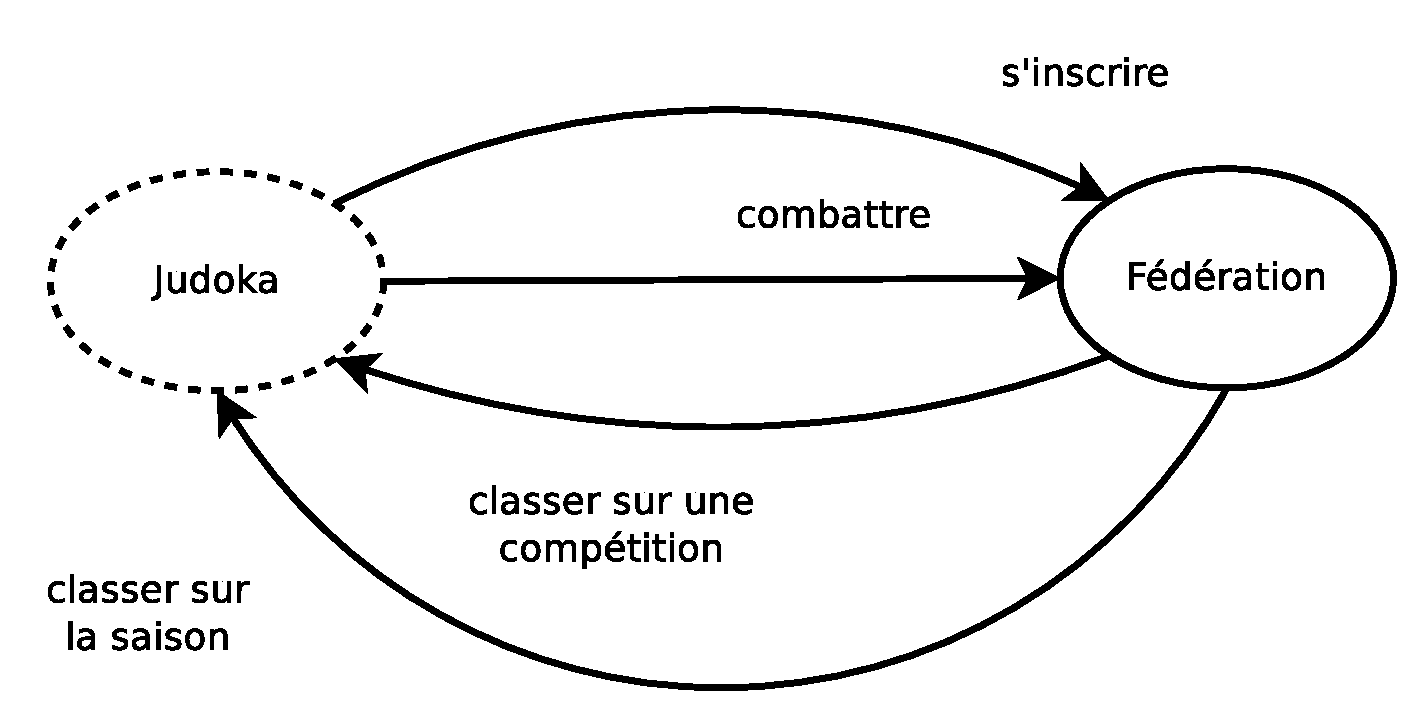
\includegraphics[width=6cm]{images/cc2_df1.eps}
    \caption{\label{cc2_df1} Diagramme de contexte}
    \end{center}
\end{figure}

\begin{figure}[!htb]
    \begin{center}
    \includegraphics[width=9cm]{images/cc2_df2.eps}
    \caption{\label{cc2_df2} Diagramme d'activités}
    \end{center}
\end{figure}

\begin{figure}[!htb]
    \begin{center}
    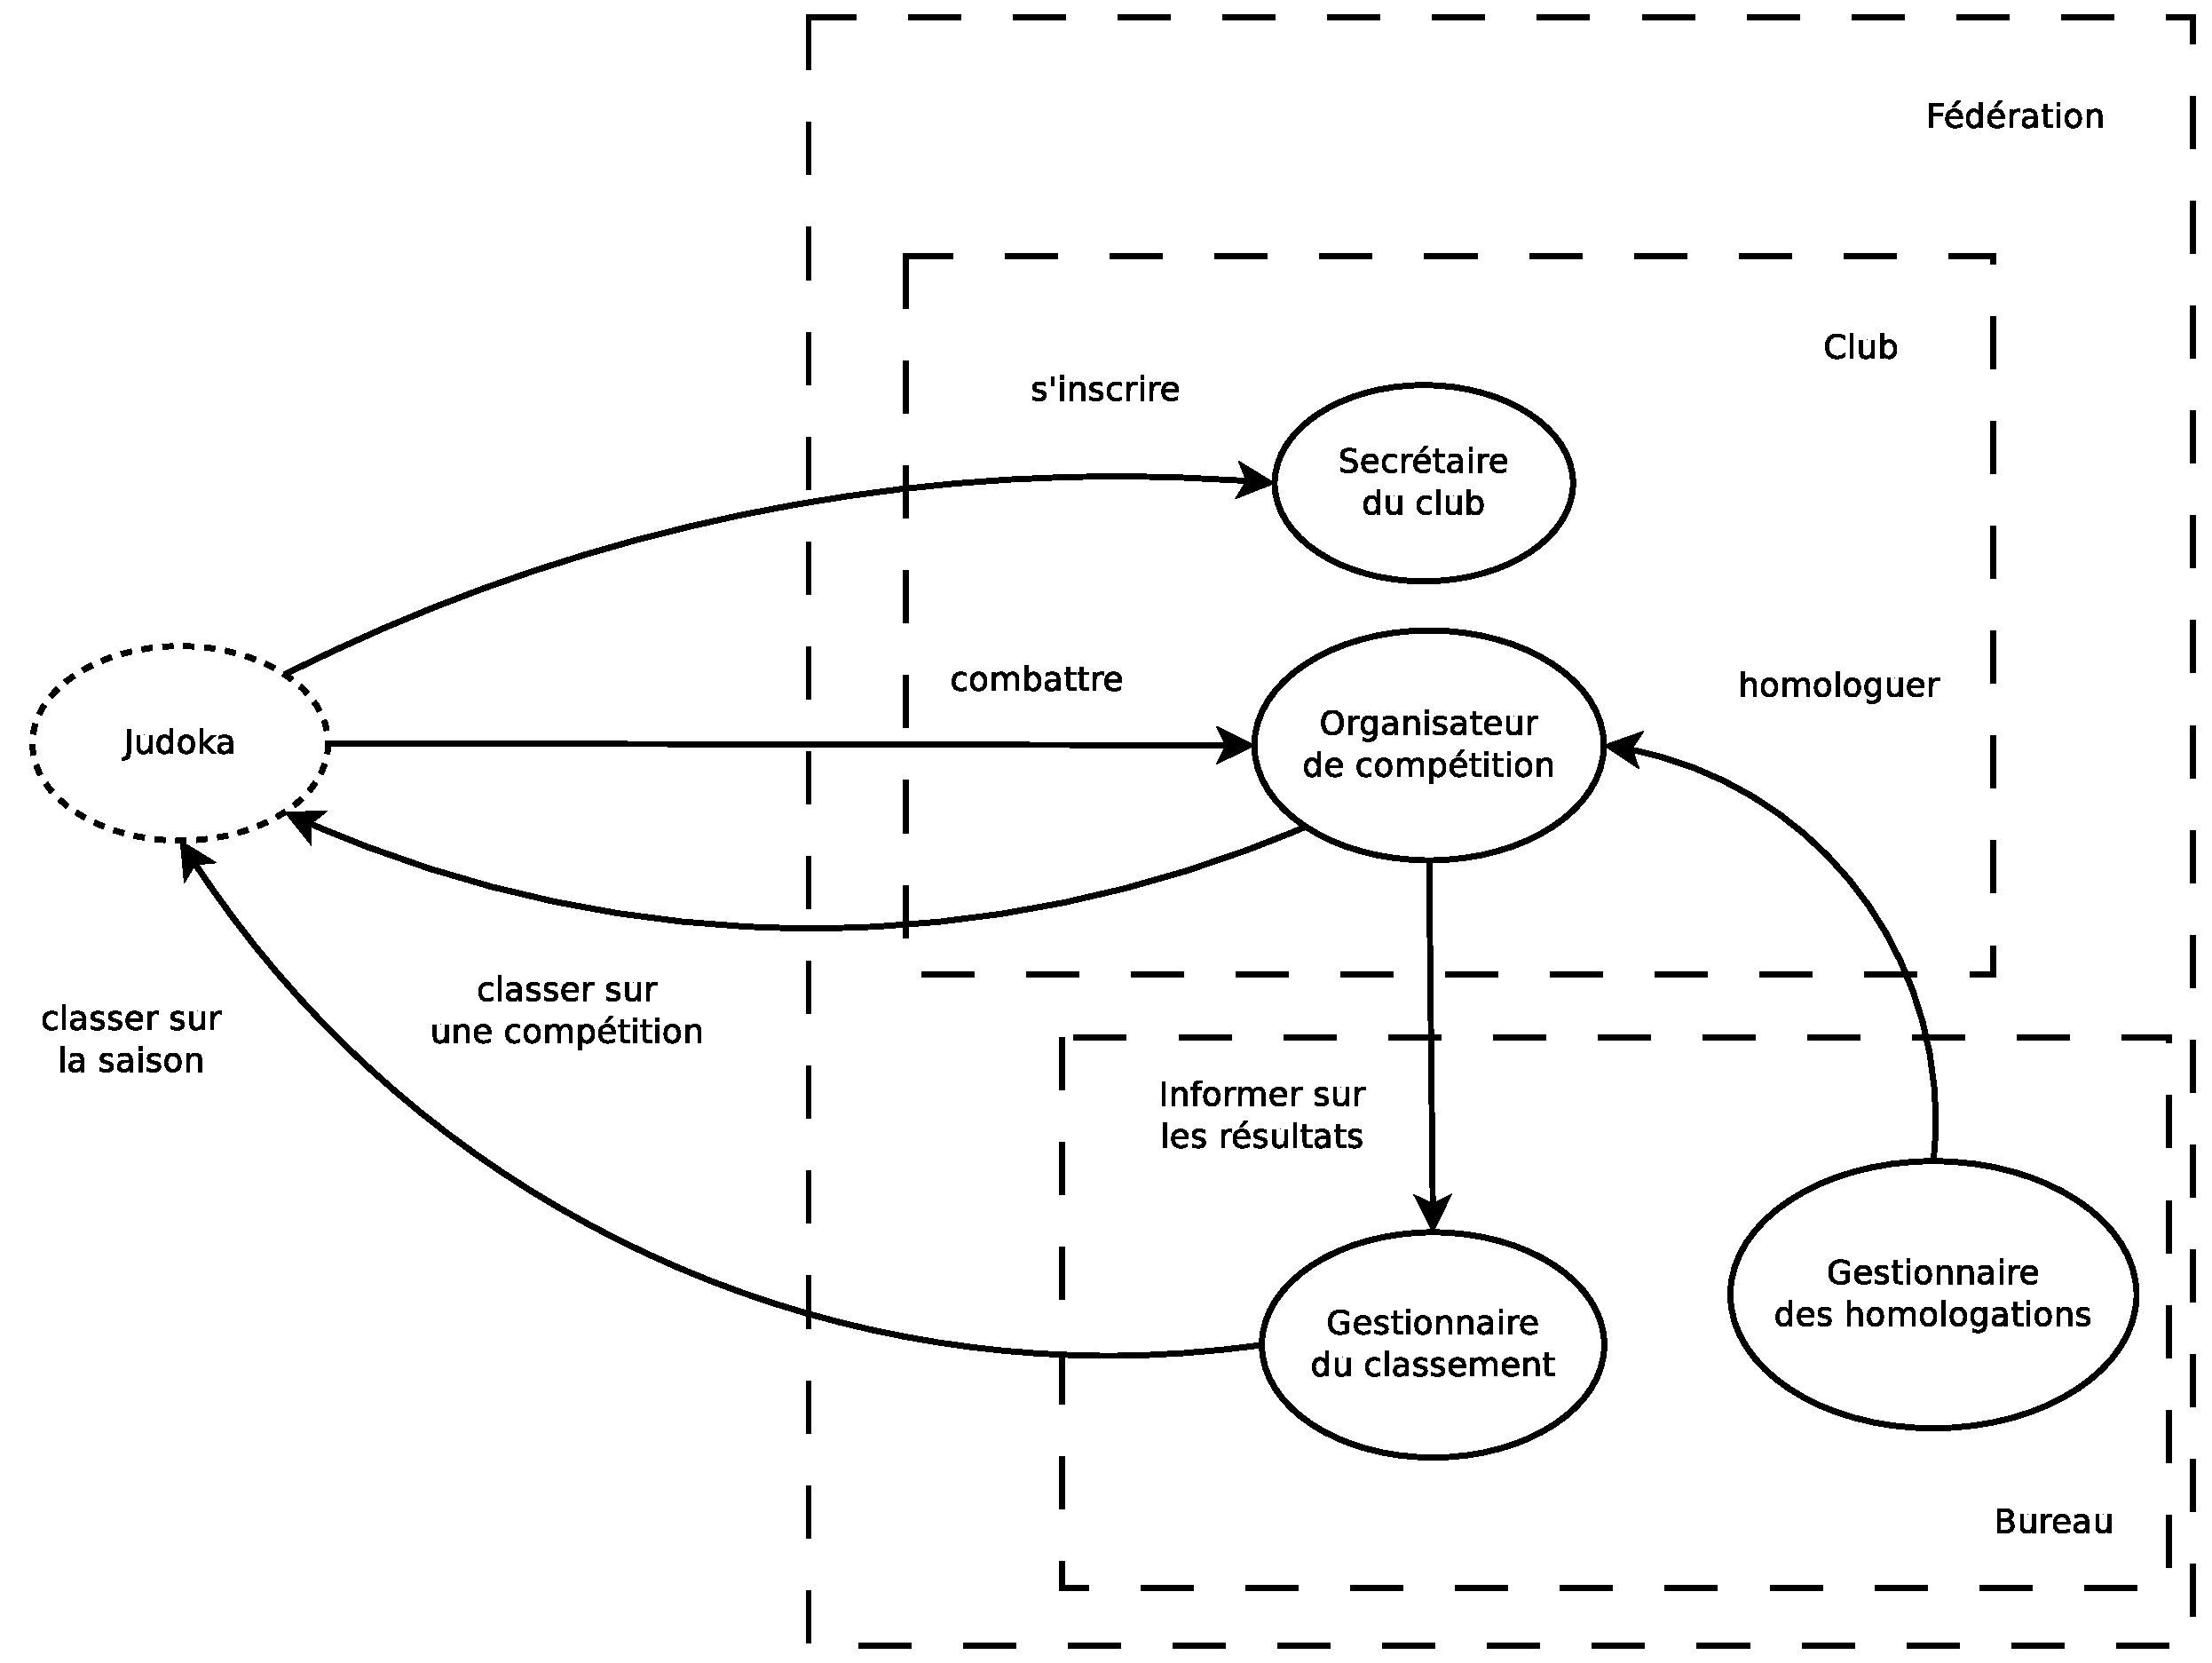
\includegraphics[width=9cm]{images/cc2_df3.eps}
    \caption{\label{cc2_df3} Diagramme de flux}
    \end{center}
\end{figure}

\section*{Matrice des Flux}

À faire à partir du diagramme de flux.

\newpage
\section*{Modèle Concptuel de Communication}

Pour chaque flux d'information du diagramme de flux, on détaille les messages échangés.

\begin{figure}[!htb]
    \begin{center}
    \includegraphics[width=6cm]{images/cc2_mcc5.eps}
    \caption{\label{cc2_mcc5} homologuer}
    \end{center}
\end{figure}

\begin{figure}[!htb]
    \begin{center}
    \includegraphics[width=6cm]{images/cc2_mcc1.eps}
    \caption{\label{cc2_mcc2} s'inscrire}
    \end{center}
\end{figure}

\begin{figure}[!htb]
    \begin{center}
    \includegraphics[width=6cm]{images/cc2_mcc2.eps}
    \caption{\label{cc2_mcc2} combattre}
    \end{center}
\end{figure}

\begin{figure}[!htb]
    \begin{center}
    \includegraphics[width=6cm]{images/cc2_mcc3.eps}
    \caption{\label{cc2_mcc3} classer sur une compétition}
    \end{center}
\end{figure}

\begin{figure}[!htb]
    \begin{center}
    \includegraphics[width=7cm]{images/cc2_mcc4.eps}
    \caption{\label{cc2_mcc4} informer sur les résultats}
    \end{center}
\end{figure}

\begin{figure}[!htb]
    \begin{center}
    \includegraphics[width=6cm]{images/cc2_mcc6.eps}
    \caption{\label{cc2_mcc5} classer sur la saison}
    \end{center}
\end{figure}

\newpage
\section*{Modèle Concptuel de Communication détaillé}

On place affecte maintenant chaque donnée du dictionnaire de données dans le message qui la contient.

\subsubsection*{demande d'homologation (Organisateur de compétition, Gestionnaire des homologations)}
\begin{itemize}
    \item nom-club
    \item adresse
\end{itemize}

\subsubsection*{homologation (Gestionnaire des homologations, Organisateur de compétition)}
\begin{itemize}
    \item année-homologation
\end{itemize}

\subsubsection*{demande d'inscription (Judoka, Secrétaire du club)}
\begin{itemize}
    \item nom-judoka
    \item sexe
    \item date-naissance
\end{itemize}

\subsubsection*{licence (Secrétaire du club, Judoka)}
\begin{itemize}
    \item no-licence
    \item nom-judoka
    \item sexe
    \item date-naissance
    \item nom-catégorie
    \item année-validité
    \item nom-club
    \item adresse
\end{itemize}

\subsubsection*{combat (Judoka, Organisateur de compétition)}
\begin{itemize}
    \item nom-compétition
    \item no-licence
\end{itemize}

\subsubsection*{feuille de match (Organisateur de compétition, Judoka)}
\begin{itemize}
    \item date-match
    \item gagnant (no-licence)
    \item perdant (no-licence)
\end{itemize}

\subsubsection*{classement compétition (Organisateur de compétition, Judoka)}
\begin{itemize}
    \item nom-compétition
    \item nom-judoka
    \item rang
\end{itemize}

\subsubsection*{feuille de match (Organisateur de compétition, Gestionnaire du classement)}
\begin{itemize}
    \item date-match
    \item gagnant (no-licence)
    \item perdant (no-licence)
\end{itemize}

\subsubsection*{classement général (Gestionnaire du classement, Judoka)}
\begin{itemize}
    \item nom-judoka
    \item nombre de victoires (calculé)
    \item nombre de défaites (calculé)
    \item points (calculé)
\end{itemize}


\newpage
\section*{Modèle Conceptuel de Données}

En suivant l'ordre des messages du MCC, on place chaque donnée véhiculée par un message dans le MCD. Pour chaque donnée, on se pose la question de l'existance d'une nouvelle entité. Une fois toutes les données placées, on valide notre MCD (formes normales).

\begin{figure}[!htb]
    \begin{center}
    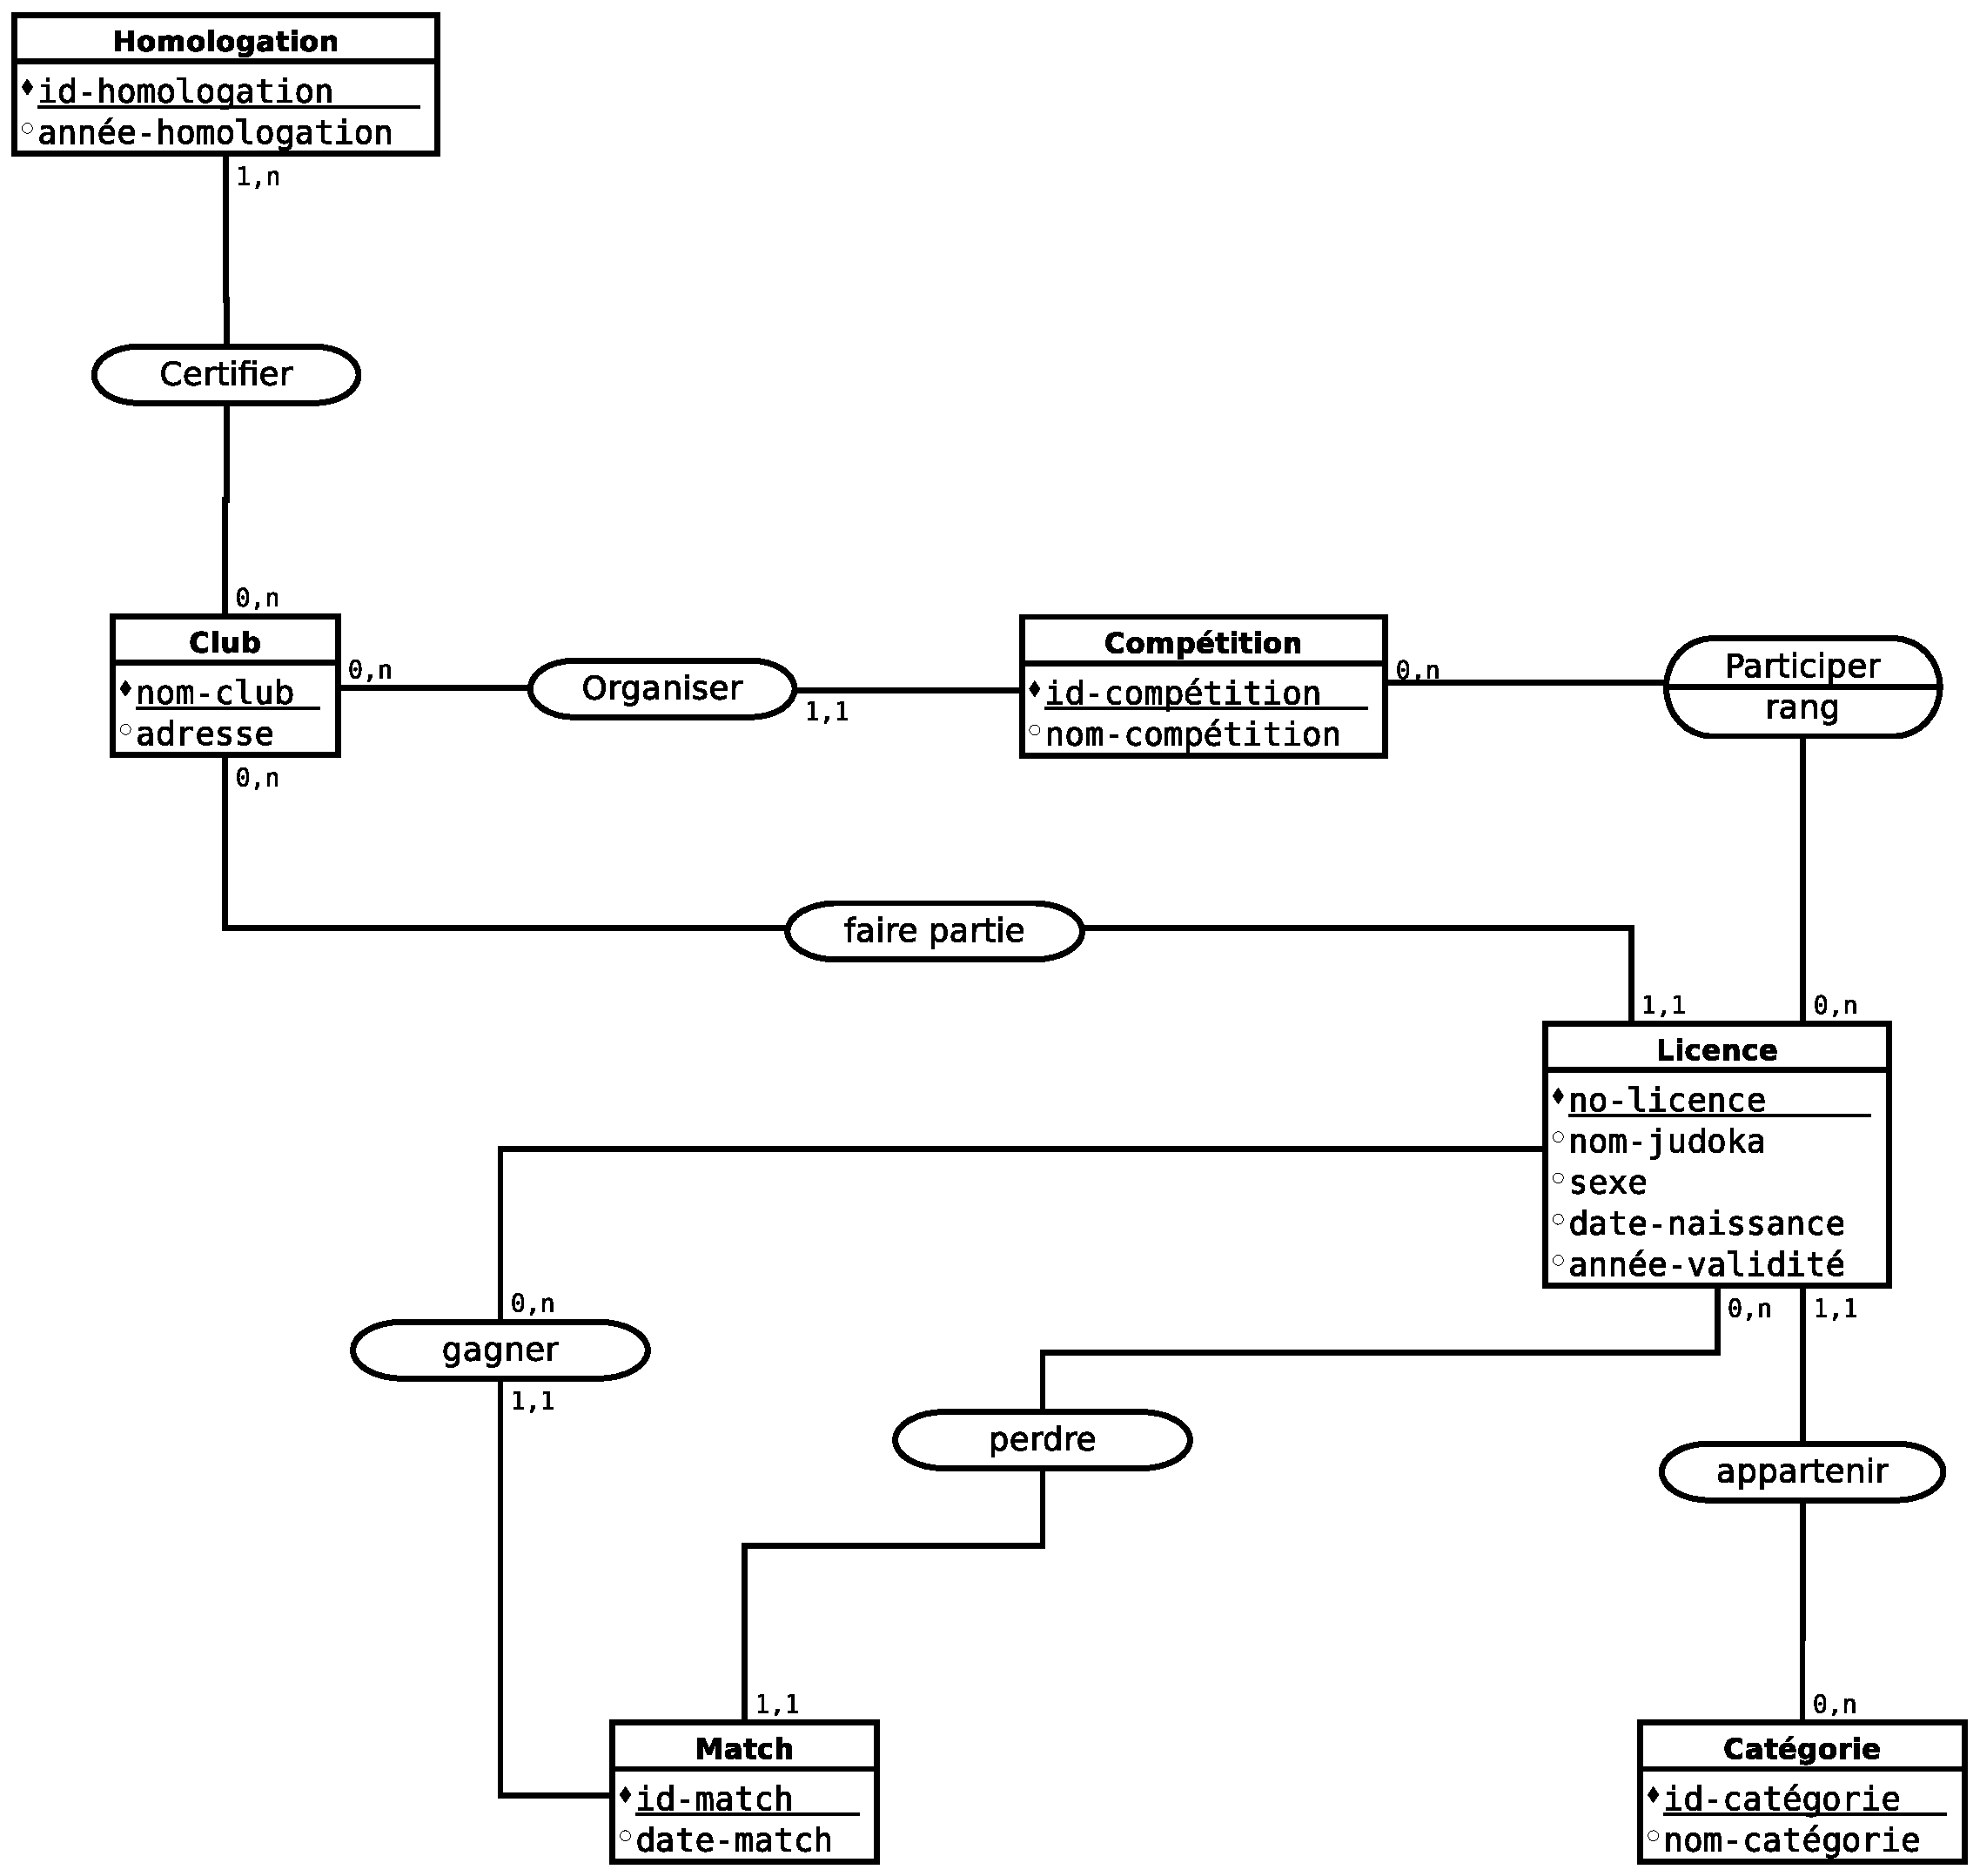
\includegraphics[width=11.5cm]{images/cc2_mcd.eps}
    \caption{\label{cc2_mcd} MCD}
    \end{center}
\end{figure}

\newpage
\section*{Modèle Conceptuel de Traitements}

Pour chaque acteur, on se demande les actions qu'il effectue sur notre système d'information.

\begin{figure}[!htb]
    \begin{center}
    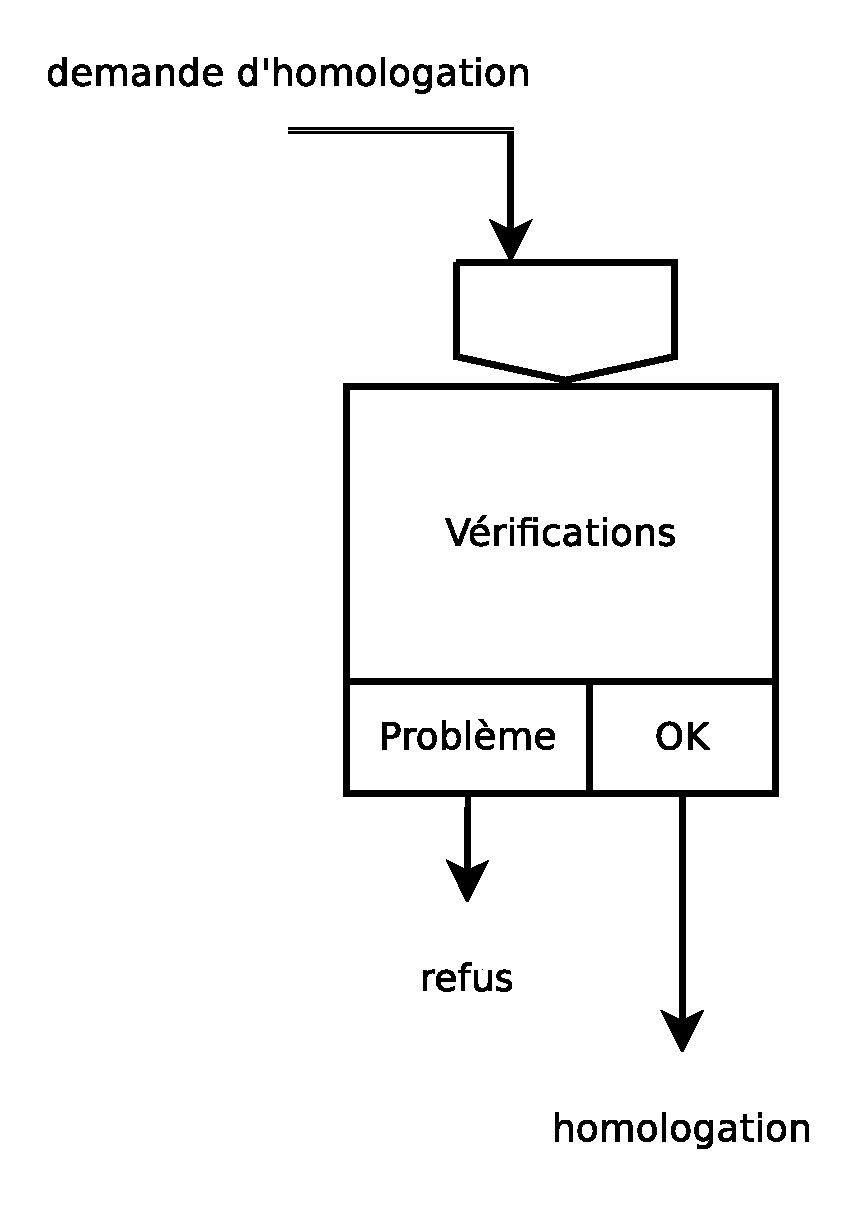
\includegraphics[height=5cm]{images/cc2_mct1.eps}
    \caption{\label{cc2_mct1} Homologation}
    \end{center}
\end{figure}

\begin{figure}[!htb]
    \begin{center}
    \includegraphics[height=5cm]{images/cc2_mct2.eps}
    \caption{\label{cc2_mct2} Inscription}
    \end{center}
\end{figure}

\begin{figure}[!htb]
    \begin{center}
    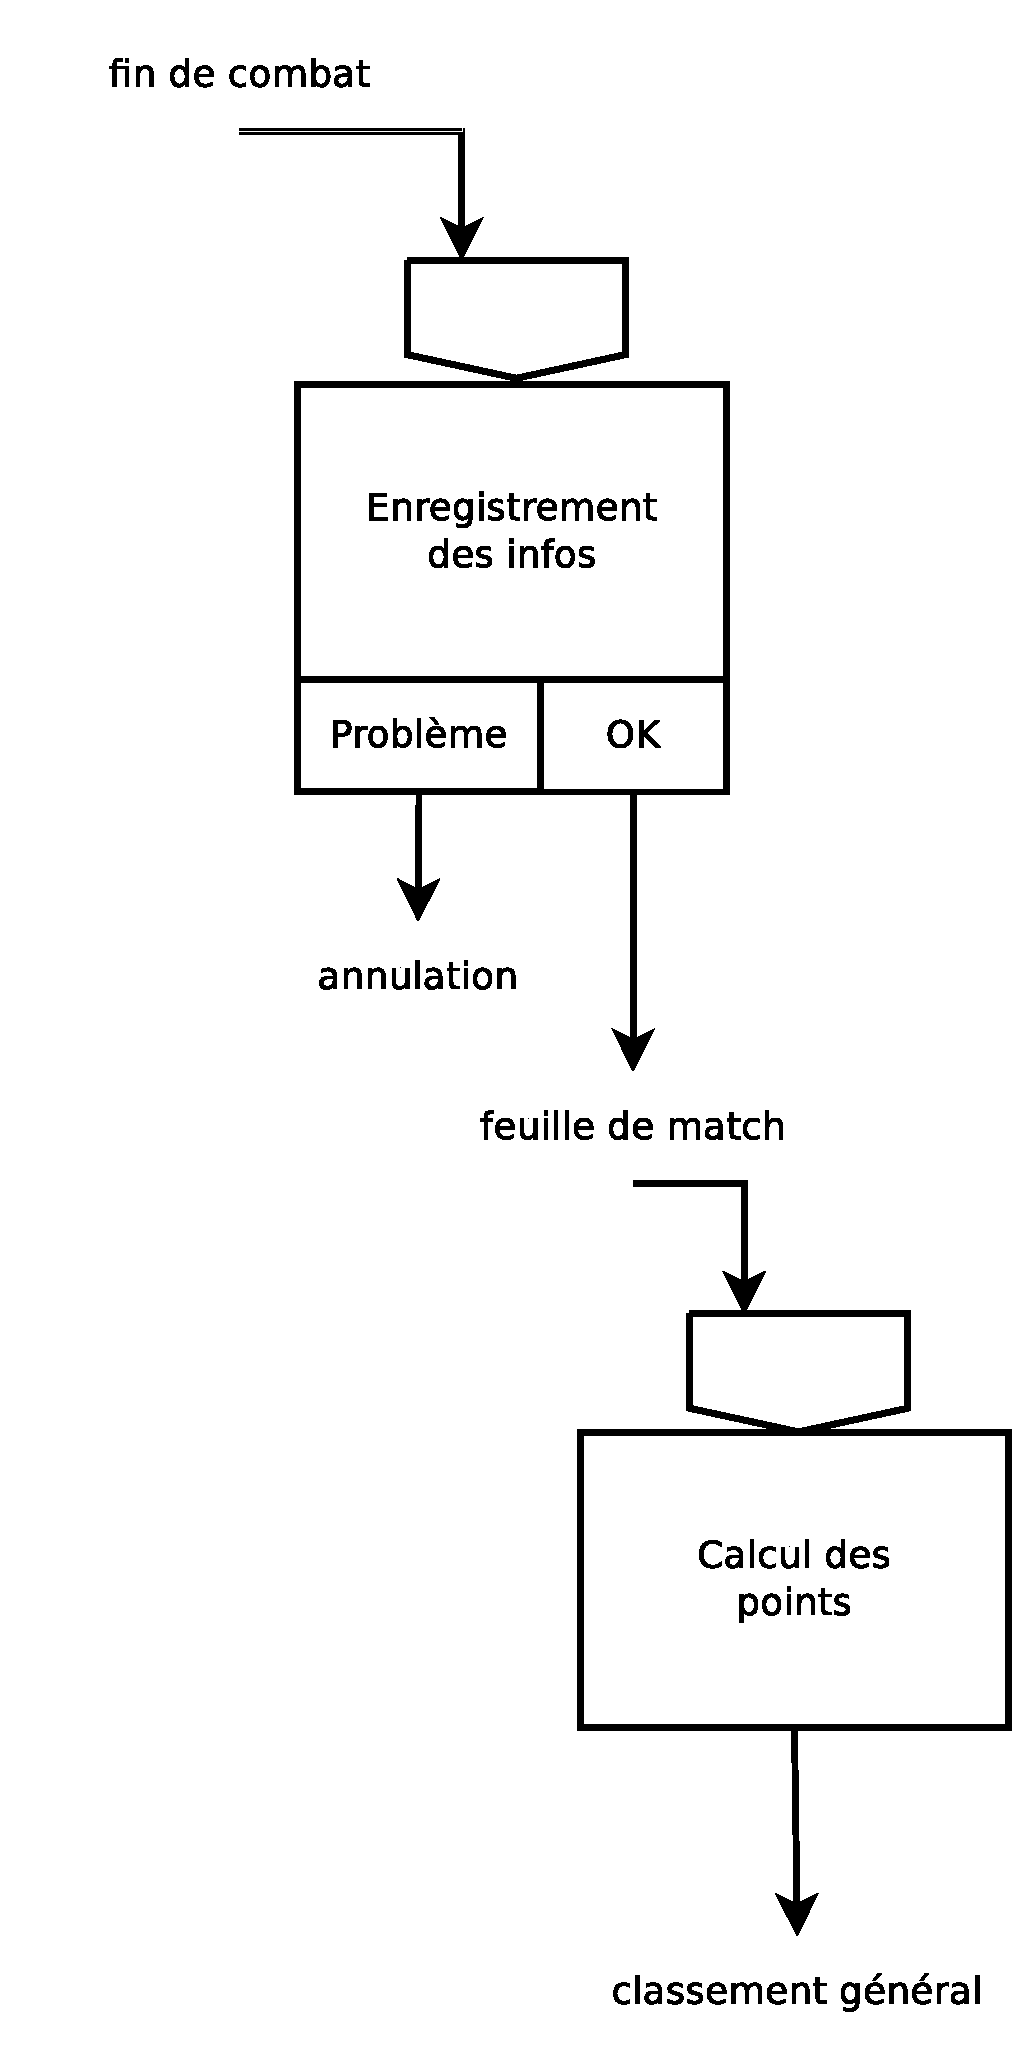
\includegraphics[height=7cm]{images/cc2_mct3.eps}
    \caption{\label{cc2_mct3} Combat et classement général}
    \end{center}
\end{figure}

\begin{figure}[!htb]
    \begin{center}
    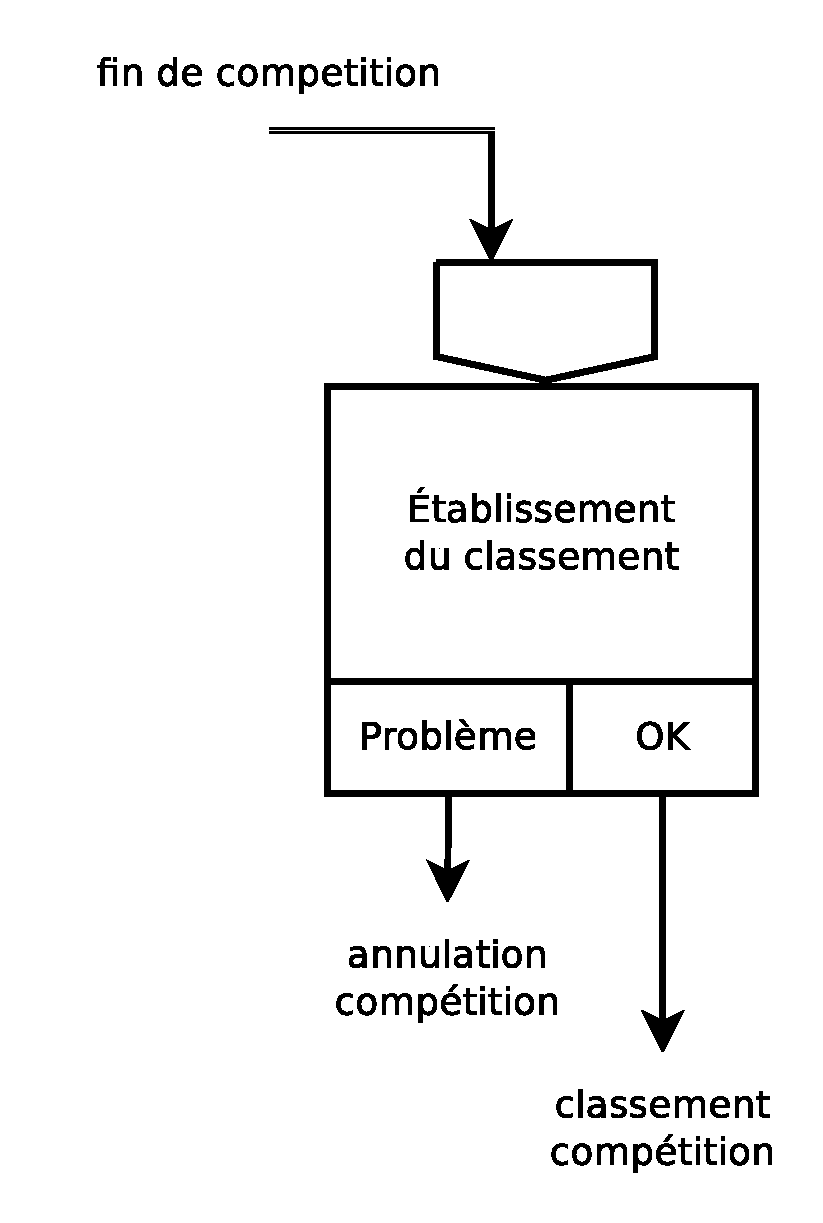
\includegraphics[height=5cm]{images/cc2_mct4.eps}
    \caption{\label{cc2_mct4} Classement compétition}
    \end{center}
\end{figure}

\newpage
\section*{Modèle Organisationel de Traitements}

On commence par déterminer les différents postes de travail d'utilisation de notre système d'information :\\

\begin{itemize}
    \item Bureau du club
    \item Bureau des homologation
    \item Bureau de classement
\end{itemize}

\begin{figure}[!htb]
    \begin{center}
    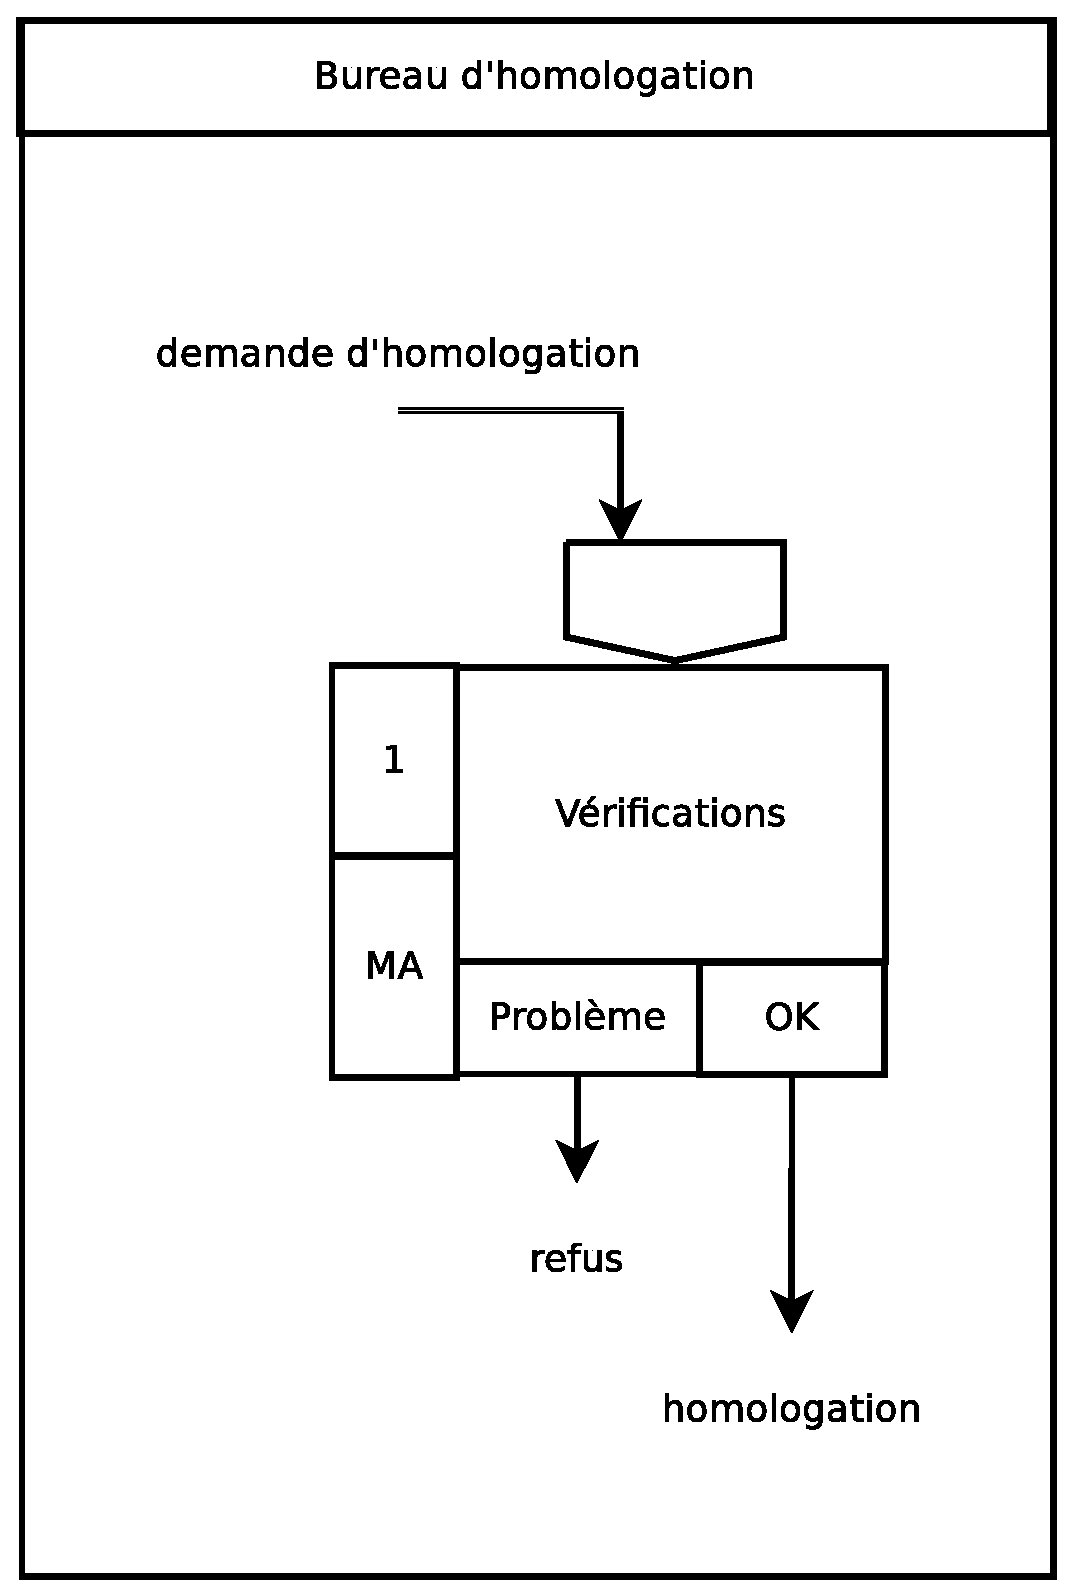
\includegraphics[height=5cm]{images/cc2_mot1.eps}
    \caption{\label{cc2_mot1} Bureau d'homologation}
    \end{center}
\end{figure}

\begin{figure}[!htb]
    \begin{center}
    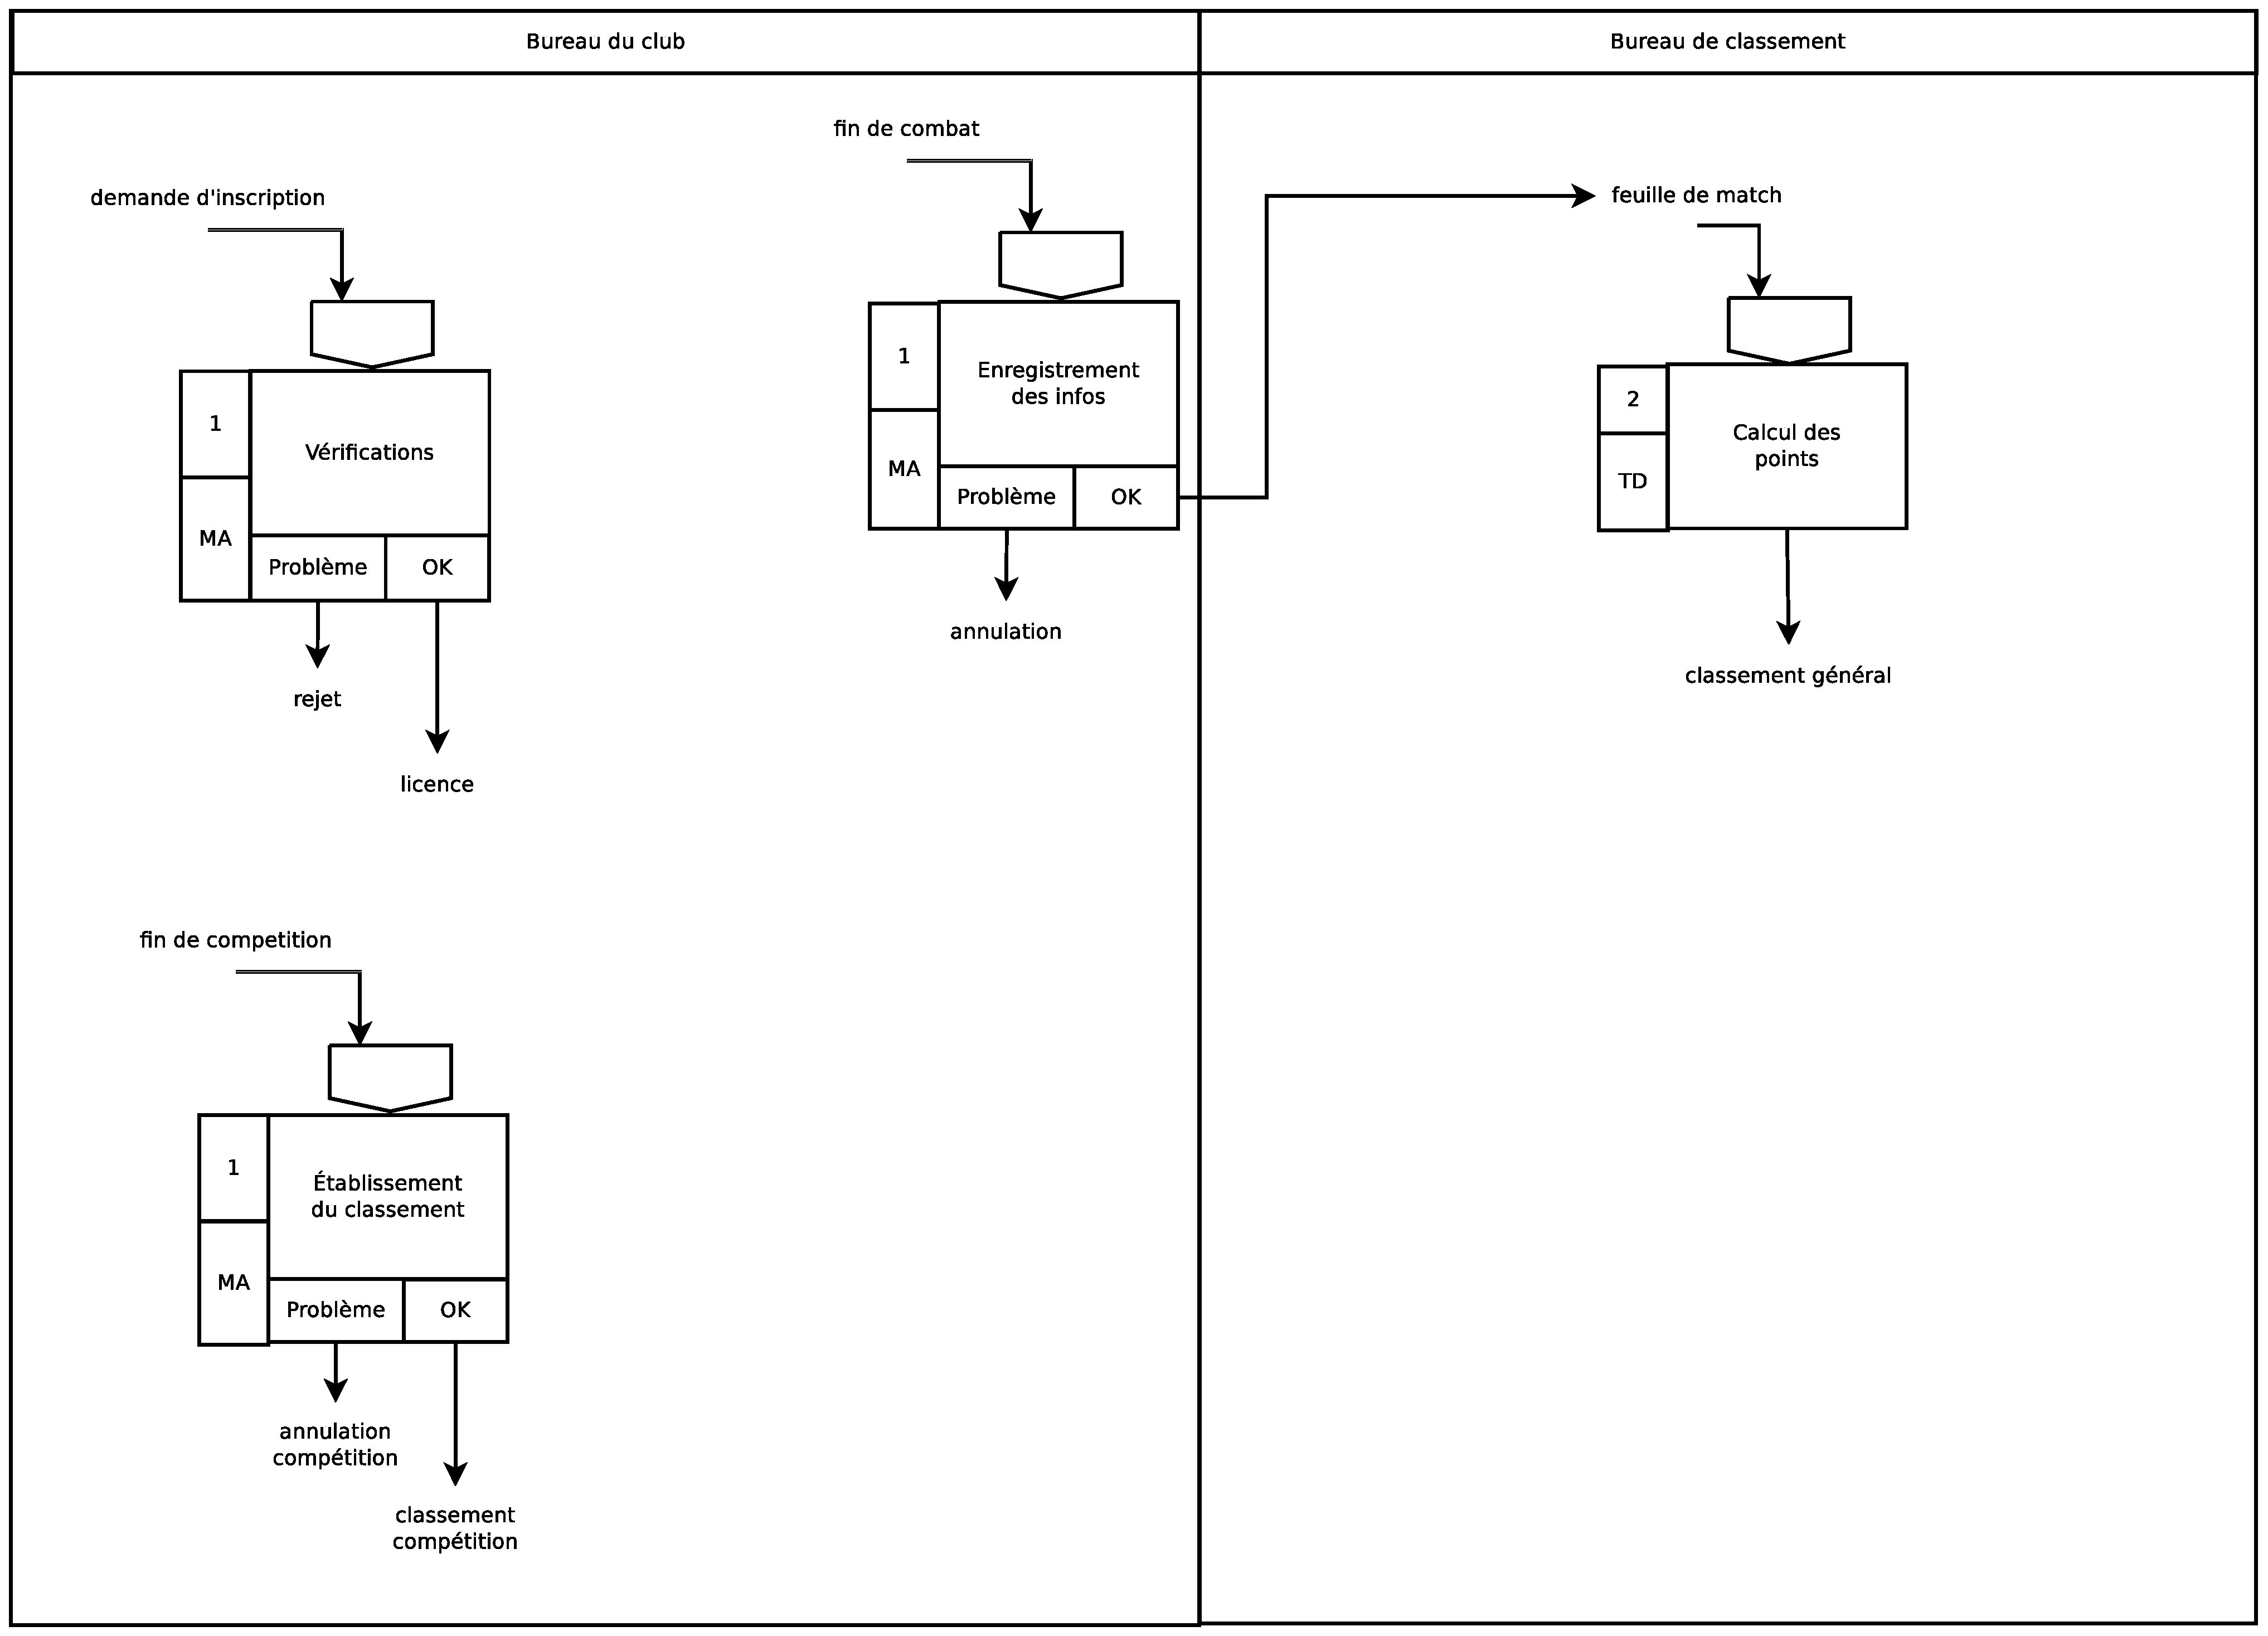
\includegraphics[height=8cm]{images/cc2_mot2.eps}
    \caption{\label{cc2_mot2} Bureau du club et bureau de classement}
    \end{center}
\end{figure}


\newpage
\section*{Modèle Organisationel de Données}

On commence par déterminer les différents sites de notre système d'information :\\

\begin{figure}[!h]
\begin{tabular}{l l}
%
    \textbf{Sites}         & \textbf{Acteurs} \\
    Salle du club          & Secrétaire du club \\
                           & Organisateur de compétition \\
    Siège de la fédération & Gestionnaire des homologations \\
                           & Gestionnaire du classement \\
%
\end{tabular}
    \caption{\label{sites} Sites}
\end{figure}

\newpage
On détermine ensuite les droits d'accès pour les entités et les asssociations porteuses de données :\\

\begin{figure}[!htb]
\begin{tabular}{| l | c | c | c | c | c | c | c | c | c | c | c | c | c | c | c | c |}
%
   \hline
                  & \multicolumn{4}{| c |}{Sec. du club} & \multicolumn{4}{| c |}{Org. de compét.} & \multicolumn{4}{| c |}{Gest. des homolog.} & \multicolumn{4}{| c |}{Gest. du class.} \\
   \hline
                  & C & L & E & S & C & L & E & S & C & L & E & S & C & L & E & S \\
   \hline
    Homologation  & - & - & - & - & - & X & - & - & X & X & X & X & - & - & - & - \\
   \hline
    Club          & - & X & - & - & - & X & - & - & X & X & X & X & - & - & - & - \\
   \hline
    Competition   & - & - & - & - & X & X & X & X & - & - & - & - & - & - & - & - \\
   \hline
    Participer    & - & - & - & - & X & X & X & X & - & - & - & - & - & - & - & - \\
   \hline
    Licence       & X & X & X & X & - & X & - & - & - & - & - & - & - & X & - & - \\ 
   \hline
    Match         & - & - & - & - & X & X & X & X & - & - & - & - & - & X & - & - \\
   \hline
    Catégorie     & - & X & - & - & X & X & X & X & - & - & - & - & - & - & - & - \\
   \hline
%
\end{tabular}
    \caption{\label{droits} Droits}
\end{figure}

\newpage
On en déduit les modèles d'organisations de données suivants : \\

\begin{figure}[!htb]
    \begin{center}
    \includegraphics[width=11.5cm]{images/cc2_mod1.eps}
    \caption{\label{cc2_mod1} MOD Salle du club}
    \end{center}
\end{figure}

\begin{figure}[!htb]
    \begin{center}
    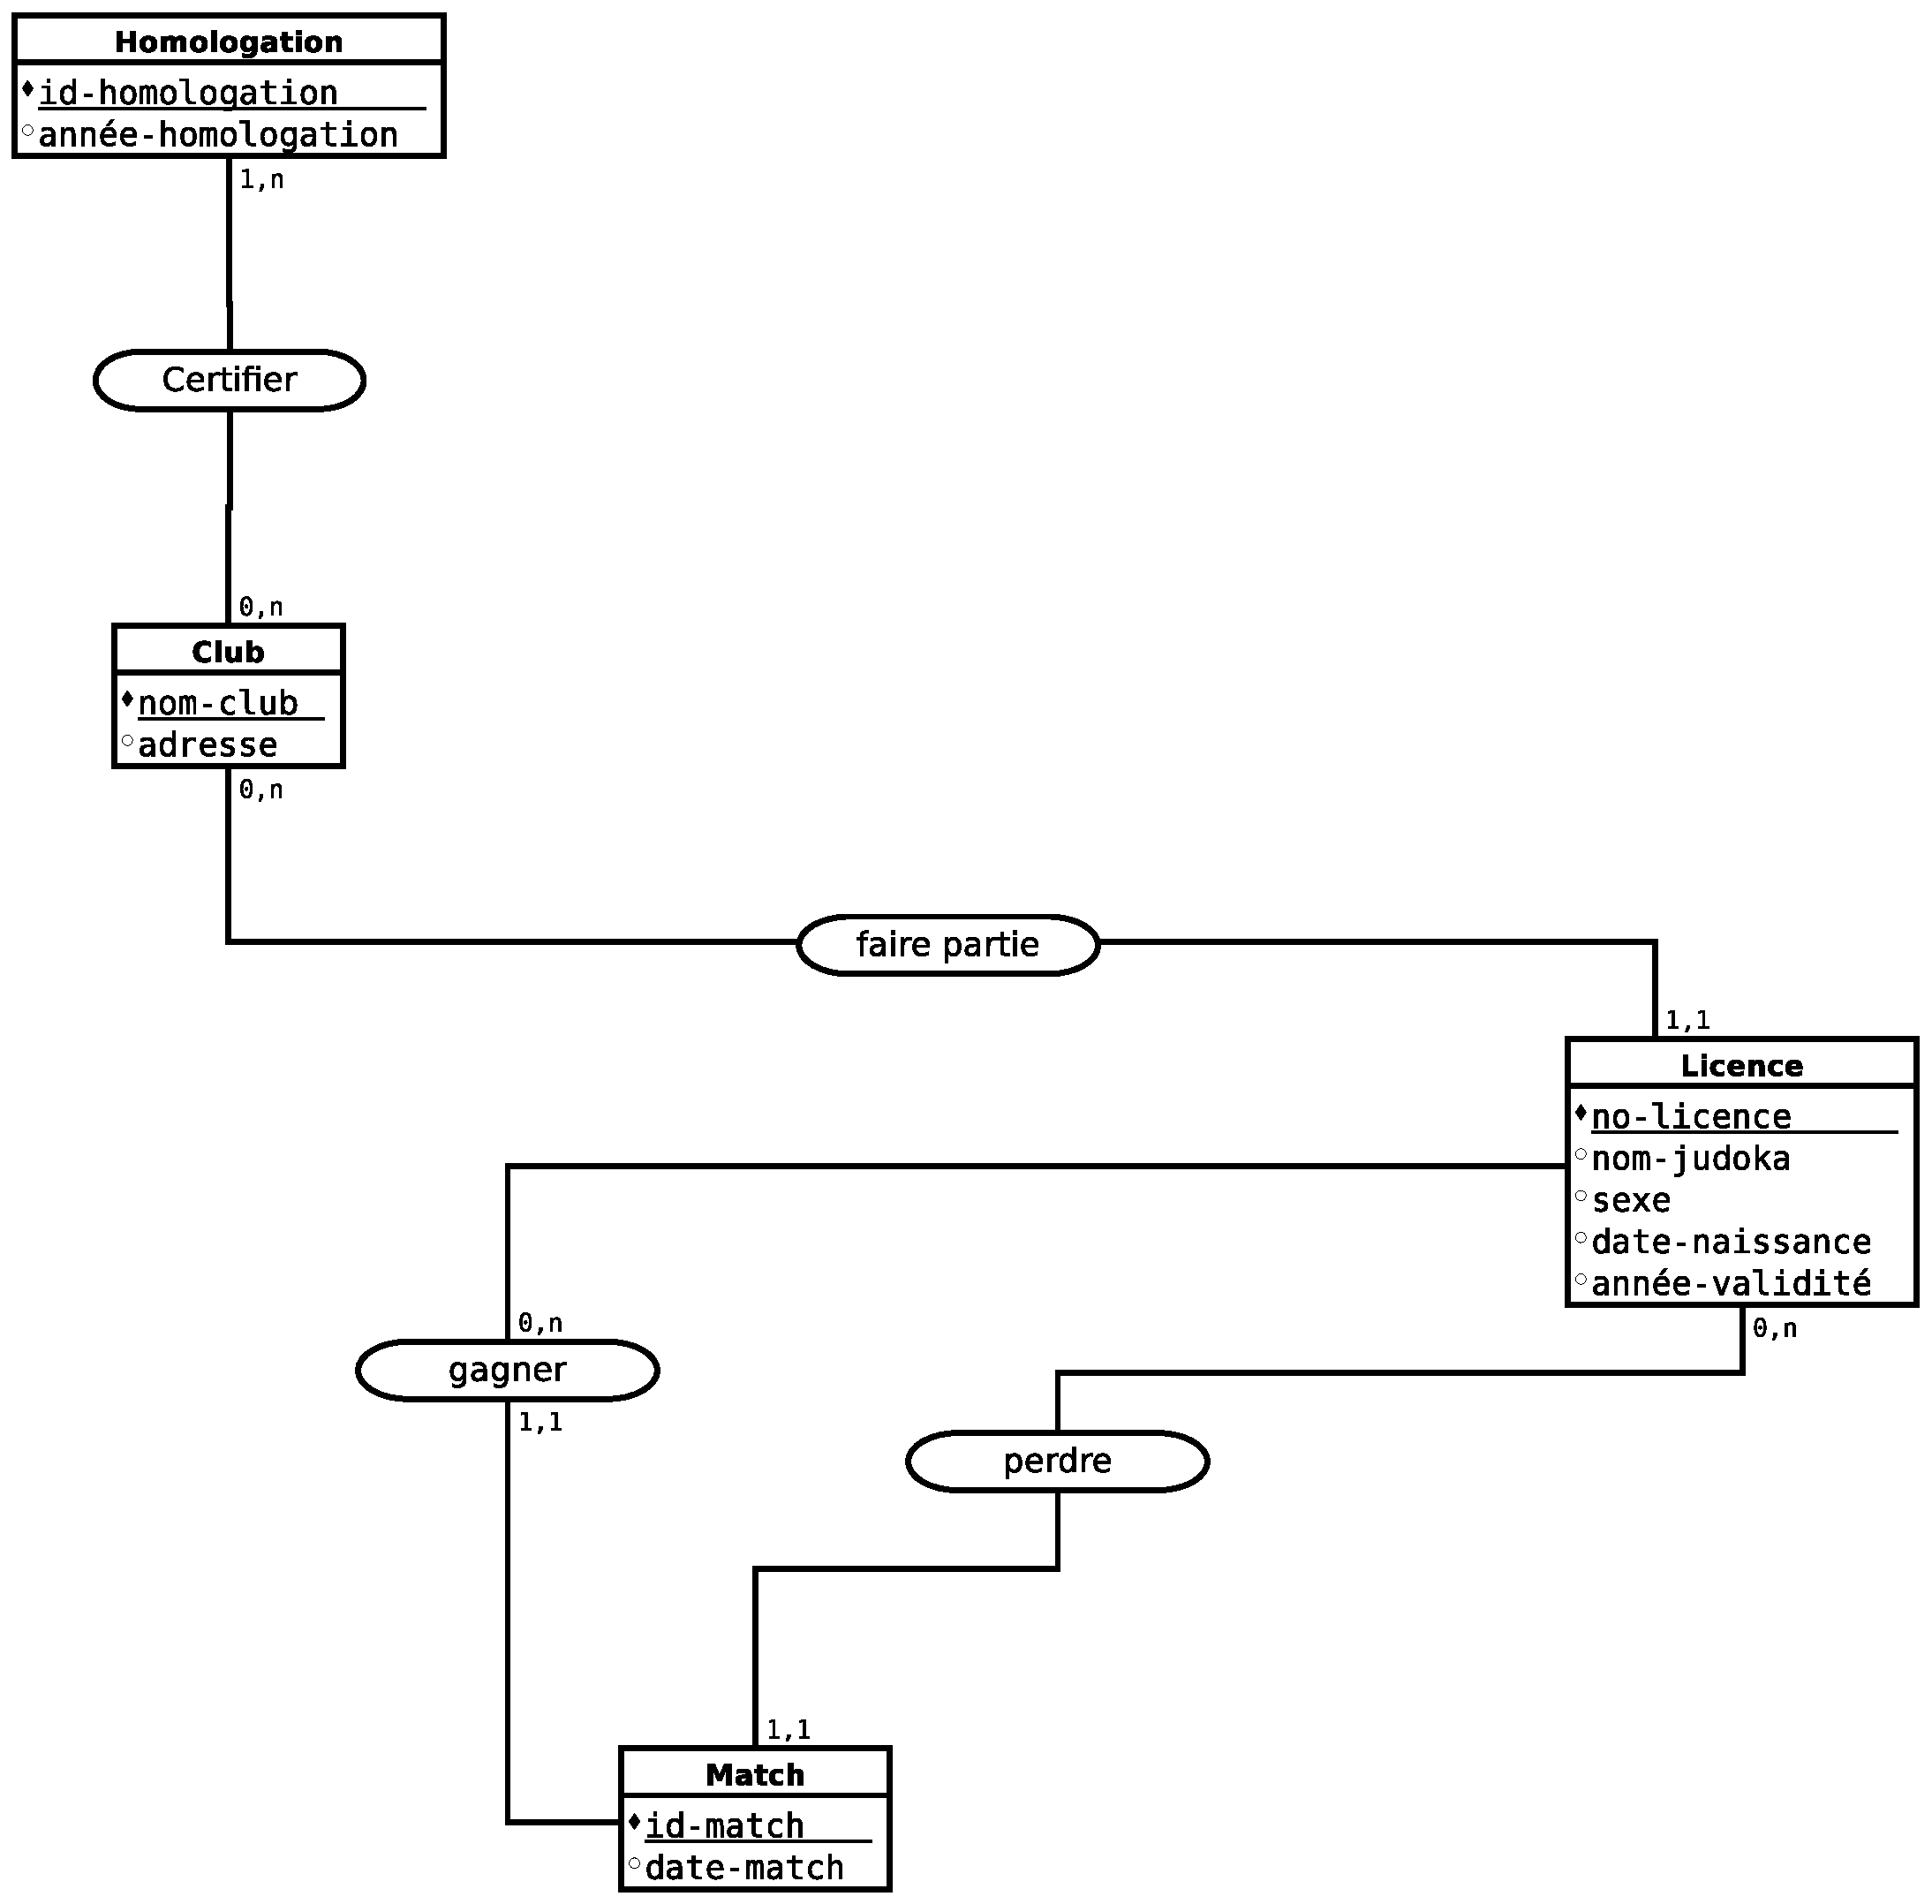
\includegraphics[width=11.5cm]{images/cc2_mod2.eps}
    \caption{\label{cc2_mod2} MOD Siège de la fédération}
    \end{center}
\end{figure}

